% Options for packages loaded elsewhere
% Options for packages loaded elsewhere
\PassOptionsToPackage{unicode}{hyperref}
\PassOptionsToPackage{hyphens}{url}
\PassOptionsToPackage{dvipsnames,svgnames,x11names}{xcolor}
%
\documentclass[
  letterpaper,
  DIV=11,
  numbers=noendperiod]{scrartcl}
\usepackage{xcolor}
\usepackage{amsmath,amssymb}
\setcounter{secnumdepth}{-\maxdimen} % remove section numbering
\usepackage{iftex}
\ifPDFTeX
  \usepackage[T1]{fontenc}
  \usepackage[utf8]{inputenc}
  \usepackage{textcomp} % provide euro and other symbols
\else % if luatex or xetex
  \usepackage{unicode-math} % this also loads fontspec
  \defaultfontfeatures{Scale=MatchLowercase}
  \defaultfontfeatures[\rmfamily]{Ligatures=TeX,Scale=1}
\fi
\usepackage{lmodern}
\ifPDFTeX\else
  % xetex/luatex font selection
\fi
% Use upquote if available, for straight quotes in verbatim environments
\IfFileExists{upquote.sty}{\usepackage{upquote}}{}
\IfFileExists{microtype.sty}{% use microtype if available
  \usepackage[]{microtype}
  \UseMicrotypeSet[protrusion]{basicmath} % disable protrusion for tt fonts
}{}
\makeatletter
\@ifundefined{KOMAClassName}{% if non-KOMA class
  \IfFileExists{parskip.sty}{%
    \usepackage{parskip}
  }{% else
    \setlength{\parindent}{0pt}
    \setlength{\parskip}{6pt plus 2pt minus 1pt}}
}{% if KOMA class
  \KOMAoptions{parskip=half}}
\makeatother
% Make \paragraph and \subparagraph free-standing
\makeatletter
\ifx\paragraph\undefined\else
  \let\oldparagraph\paragraph
  \renewcommand{\paragraph}{
    \@ifstar
      \xxxParagraphStar
      \xxxParagraphNoStar
  }
  \newcommand{\xxxParagraphStar}[1]{\oldparagraph*{#1}\mbox{}}
  \newcommand{\xxxParagraphNoStar}[1]{\oldparagraph{#1}\mbox{}}
\fi
\ifx\subparagraph\undefined\else
  \let\oldsubparagraph\subparagraph
  \renewcommand{\subparagraph}{
    \@ifstar
      \xxxSubParagraphStar
      \xxxSubParagraphNoStar
  }
  \newcommand{\xxxSubParagraphStar}[1]{\oldsubparagraph*{#1}\mbox{}}
  \newcommand{\xxxSubParagraphNoStar}[1]{\oldsubparagraph{#1}\mbox{}}
\fi
\makeatother

\usepackage{color}
\usepackage{fancyvrb}
\newcommand{\VerbBar}{|}
\newcommand{\VERB}{\Verb[commandchars=\\\{\}]}
\DefineVerbatimEnvironment{Highlighting}{Verbatim}{commandchars=\\\{\}}
% Add ',fontsize=\small' for more characters per line
\usepackage{framed}
\definecolor{shadecolor}{RGB}{241,243,245}
\newenvironment{Shaded}{\begin{snugshade}}{\end{snugshade}}
\newcommand{\AlertTok}[1]{\textcolor[rgb]{0.68,0.00,0.00}{#1}}
\newcommand{\AnnotationTok}[1]{\textcolor[rgb]{0.37,0.37,0.37}{#1}}
\newcommand{\AttributeTok}[1]{\textcolor[rgb]{0.40,0.45,0.13}{#1}}
\newcommand{\BaseNTok}[1]{\textcolor[rgb]{0.68,0.00,0.00}{#1}}
\newcommand{\BuiltInTok}[1]{\textcolor[rgb]{0.00,0.23,0.31}{#1}}
\newcommand{\CharTok}[1]{\textcolor[rgb]{0.13,0.47,0.30}{#1}}
\newcommand{\CommentTok}[1]{\textcolor[rgb]{0.37,0.37,0.37}{#1}}
\newcommand{\CommentVarTok}[1]{\textcolor[rgb]{0.37,0.37,0.37}{\textit{#1}}}
\newcommand{\ConstantTok}[1]{\textcolor[rgb]{0.56,0.35,0.01}{#1}}
\newcommand{\ControlFlowTok}[1]{\textcolor[rgb]{0.00,0.23,0.31}{\textbf{#1}}}
\newcommand{\DataTypeTok}[1]{\textcolor[rgb]{0.68,0.00,0.00}{#1}}
\newcommand{\DecValTok}[1]{\textcolor[rgb]{0.68,0.00,0.00}{#1}}
\newcommand{\DocumentationTok}[1]{\textcolor[rgb]{0.37,0.37,0.37}{\textit{#1}}}
\newcommand{\ErrorTok}[1]{\textcolor[rgb]{0.68,0.00,0.00}{#1}}
\newcommand{\ExtensionTok}[1]{\textcolor[rgb]{0.00,0.23,0.31}{#1}}
\newcommand{\FloatTok}[1]{\textcolor[rgb]{0.68,0.00,0.00}{#1}}
\newcommand{\FunctionTok}[1]{\textcolor[rgb]{0.28,0.35,0.67}{#1}}
\newcommand{\ImportTok}[1]{\textcolor[rgb]{0.00,0.46,0.62}{#1}}
\newcommand{\InformationTok}[1]{\textcolor[rgb]{0.37,0.37,0.37}{#1}}
\newcommand{\KeywordTok}[1]{\textcolor[rgb]{0.00,0.23,0.31}{\textbf{#1}}}
\newcommand{\NormalTok}[1]{\textcolor[rgb]{0.00,0.23,0.31}{#1}}
\newcommand{\OperatorTok}[1]{\textcolor[rgb]{0.37,0.37,0.37}{#1}}
\newcommand{\OtherTok}[1]{\textcolor[rgb]{0.00,0.23,0.31}{#1}}
\newcommand{\PreprocessorTok}[1]{\textcolor[rgb]{0.68,0.00,0.00}{#1}}
\newcommand{\RegionMarkerTok}[1]{\textcolor[rgb]{0.00,0.23,0.31}{#1}}
\newcommand{\SpecialCharTok}[1]{\textcolor[rgb]{0.37,0.37,0.37}{#1}}
\newcommand{\SpecialStringTok}[1]{\textcolor[rgb]{0.13,0.47,0.30}{#1}}
\newcommand{\StringTok}[1]{\textcolor[rgb]{0.13,0.47,0.30}{#1}}
\newcommand{\VariableTok}[1]{\textcolor[rgb]{0.07,0.07,0.07}{#1}}
\newcommand{\VerbatimStringTok}[1]{\textcolor[rgb]{0.13,0.47,0.30}{#1}}
\newcommand{\WarningTok}[1]{\textcolor[rgb]{0.37,0.37,0.37}{\textit{#1}}}

\usepackage{longtable,booktabs,array}
\usepackage{calc} % for calculating minipage widths
% Correct order of tables after \paragraph or \subparagraph
\usepackage{etoolbox}
\makeatletter
\patchcmd\longtable{\par}{\if@noskipsec\mbox{}\fi\par}{}{}
\makeatother
% Allow footnotes in longtable head/foot
\IfFileExists{footnotehyper.sty}{\usepackage{footnotehyper}}{\usepackage{footnote}}
\makesavenoteenv{longtable}
\usepackage{graphicx}
\makeatletter
\newsavebox\pandoc@box
\newcommand*\pandocbounded[1]{% scales image to fit in text height/width
  \sbox\pandoc@box{#1}%
  \Gscale@div\@tempa{\textheight}{\dimexpr\ht\pandoc@box+\dp\pandoc@box\relax}%
  \Gscale@div\@tempb{\linewidth}{\wd\pandoc@box}%
  \ifdim\@tempb\p@<\@tempa\p@\let\@tempa\@tempb\fi% select the smaller of both
  \ifdim\@tempa\p@<\p@\scalebox{\@tempa}{\usebox\pandoc@box}%
  \else\usebox{\pandoc@box}%
  \fi%
}
% Set default figure placement to htbp
\def\fps@figure{htbp}
\makeatother


% definitions for citeproc citations
\NewDocumentCommand\citeproctext{}{}
\NewDocumentCommand\citeproc{mm}{%
  \begingroup\def\citeproctext{#2}\cite{#1}\endgroup}
\makeatletter
 % allow citations to break across lines
 \let\@cite@ofmt\@firstofone
 % avoid brackets around text for \cite:
 \def\@biblabel#1{}
 \def\@cite#1#2{{#1\if@tempswa , #2\fi}}
\makeatother
\newlength{\cslhangindent}
\setlength{\cslhangindent}{1.5em}
\newlength{\csllabelwidth}
\setlength{\csllabelwidth}{3em}
\newenvironment{CSLReferences}[2] % #1 hanging-indent, #2 entry-spacing
 {\begin{list}{}{%
  \setlength{\itemindent}{0pt}
  \setlength{\leftmargin}{0pt}
  \setlength{\parsep}{0pt}
  % turn on hanging indent if param 1 is 1
  \ifodd #1
   \setlength{\leftmargin}{\cslhangindent}
   \setlength{\itemindent}{-1\cslhangindent}
  \fi
  % set entry spacing
  \setlength{\itemsep}{#2\baselineskip}}}
 {\end{list}}
\usepackage{calc}
\newcommand{\CSLBlock}[1]{\hfill\break\parbox[t]{\linewidth}{\strut\ignorespaces#1\strut}}
\newcommand{\CSLLeftMargin}[1]{\parbox[t]{\csllabelwidth}{\strut#1\strut}}
\newcommand{\CSLRightInline}[1]{\parbox[t]{\linewidth - \csllabelwidth}{\strut#1\strut}}
\newcommand{\CSLIndent}[1]{\hspace{\cslhangindent}#1}



\setlength{\emergencystretch}{3em} % prevent overfull lines

\providecommand{\tightlist}{%
  \setlength{\itemsep}{0pt}\setlength{\parskip}{0pt}}



 


\KOMAoption{captions}{tableheading}
\makeatletter
\@ifpackageloaded{caption}{}{\usepackage{caption}}
\AtBeginDocument{%
\ifdefined\contentsname
  \renewcommand*\contentsname{Table of contents}
\else
  \newcommand\contentsname{Table of contents}
\fi
\ifdefined\listfigurename
  \renewcommand*\listfigurename{List of Figures}
\else
  \newcommand\listfigurename{List of Figures}
\fi
\ifdefined\listtablename
  \renewcommand*\listtablename{List of Tables}
\else
  \newcommand\listtablename{List of Tables}
\fi
\ifdefined\figurename
  \renewcommand*\figurename{Figure}
\else
  \newcommand\figurename{Figure}
\fi
\ifdefined\tablename
  \renewcommand*\tablename{Table}
\else
  \newcommand\tablename{Table}
\fi
}
\@ifpackageloaded{float}{}{\usepackage{float}}
\floatstyle{ruled}
\@ifundefined{c@chapter}{\newfloat{codelisting}{h}{lop}}{\newfloat{codelisting}{h}{lop}[chapter]}
\floatname{codelisting}{Listing}
\newcommand*\listoflistings{\listof{codelisting}{List of Listings}}
\makeatother
\makeatletter
\makeatother
\makeatletter
\@ifpackageloaded{caption}{}{\usepackage{caption}}
\@ifpackageloaded{subcaption}{}{\usepackage{subcaption}}
\makeatother
\usepackage{bookmark}
\IfFileExists{xurl.sty}{\usepackage{xurl}}{} % add URL line breaks if available
\urlstyle{same}
\hypersetup{
  pdftitle={Analysis of iPSC Gene Expression (will be changed)},
  pdfauthor={Trinity Minard},
  colorlinks=true,
  linkcolor={blue},
  filecolor={Maroon},
  citecolor={Blue},
  urlcolor={Blue},
  pdfcreator={LaTeX via pandoc}}


\title{Analysis of iPSC Gene Expression (will be changed)}
\usepackage{etoolbox}
\makeatletter
\providecommand{\subtitle}[1]{% add subtitle to \maketitle
  \apptocmd{\@title}{\par {\large #1 \par}}{}{}
}
\makeatother
\subtitle{Final Project}
\author{Trinity Minard}
\date{2025-11-19}
\begin{document}
\maketitle


\section{Introduction}\label{introduction}

The discovery of human induced pluripotent stem cells (iPSCs) by
Takahashi and Yamanaka in 2007 (Takahashi et al., 2007) has
revolutionized the regenerative medicine field. iPSCs are created by
reprogramming somatic cells into an embryonic like state using the
Yamanaka transciption factors: SOX2, OCT4, KLF4, and c-Myc). These cells
have vast capabilities due to their ability to model human development
and diseases \emph{in vitro}, and their potential for patient specific
(autologous) and ``off the shelf'' (allogeneic) cell therapies
(Cerneckis et al., 2024).

With that being said, the characterization of iPSC lines is essential in
any experimental or manufacturing process to ensure consistency in
culturing. This includes analyzing the expression of pluripotency (stem
cell) markers, differentiation markers, and potential chromosomal
abnormalies, to access the population of the culture. This is commonly
done using techniques such as reverse transcriptase or real time
quantitative PCR (RT-qPCR) to analyze mRNA expression (Artyukhov et al.,
2017), or using an antibody based experiment to analyze protein
expression levels, such as Flow Cytometry or immunocytochemistry. When
conducting these experiments, specifically RT-qPCR, reference genes,
also known as housekeeping genes, are used to normalize the expression
of other genes in a sample (Artyukhov et al., 2017). This allows the
expression of genes to be compared across different samples, since it is
presumed that the expression of the housekeeping gene is consistent
across all of the samples. In stem cell samples, however, it has been
found that the commonly used housekeeping genes, such as GAPDH, appear
to fluctuate in iPSC samples (Panina et al., 2020), making it difficult
to achieve accurate normalization data.

RNA Seq is a technique that sequences the entirety of RNA molecules in a
given sample, rather than using gene specific primers or probes as in
RT-qPCR and other techniques. This allows the entire transciptome to be
analyzed, providing a complete picture of the expression of genes in a
sample (Wang et al., 2009). Additionally, gene expression is calculated
by dividing the raw counts of a gene by the total counts in a sample,
eliminating the need for a housekeeping gene. This allows for an
unbiased and quantitiative analysis of millions of genes in sample (Wang
et al., 2009). Despite these advantages, RNA-Seq is far more time
consuming and expensive than RT-qPCR and other experiments, making it
non practical in a manufacturing setting. Therefore, utilizing RNA-Seq
to analyze iPSC samples could provide insight into housekeeping gene
expression, allowing researchers to select ideal reference genes for
their analysis.

A similar study, conducted by Carcamo-Orive \emph{et al.,} investigated
the variability of gene expression across 317 iPSC lines generated from
101 individuals (Carcamo-Orive et al., 2017) and created a publically
avaible data set of their raw RNA Seq data. They found that genetic
variability in the iPSC lines was influenced by a donor specific gene
expression pattern, specifically influenced by donor age, sex, ancestry,
and reprogramming variabilies. iPSCs can also be reprogrammed from a
variety of somatic cells, such as blood, skin fibroblasts, hair
keratinocytes, urine cells, mesencymal stem cells, and bone marrow
(Poetsch et al., 2022). While some somatic cells are easier to obtain
than others, such as blood cells and fibroblasts, iPSCs from these lines
are associated with higher genomic mutations due to the somatic cells'
high turnover rate. Additionally, iPSCs appear to have an epigenetic
memory of their tissue of origin, which has been found to influence
their differentiation (Poetsch et al., 2022). All of these factors, and
many others, could be contributing to the variations in gene expression
in iPSC samples.

This publicly available dataset from Carcamo-Orive \emph{et al.} was
used to analyze the expression of RNA across iPSC samples, with a focus
on the expression of pluripotency markers, differentiation markers, and
housekeeping genes.

\section{Methods}\label{methods}

\subsubsection{Data Cleaning}\label{data-cleaning}

RNA-Seq counts per million data was acquired from Stemformatics
(\emph{Stemformatics Datasets}, n.d.), using the Carcamo-Orive (2017)
dataset (Carcamo-Orive et al., 2017). Genes in this study were referred
to by their Ensembl ID, so gene information was integrated from Emsembl
database (\emph{Ensembl Biomart}, n.d.). To begin to clean the data, the
Ensembl gene ID in both the count per million data frame and Ensembl
data frame were mutated, using the dplyr package (Wickham et al., 2023)
from tidyverse (Wickham, 2023), to the name: Gene stable ID. The Ensembl
gene data frame was then filtered for the genes in the count per million
data set (reducing the number of genes from 86,369 to 56,693).

\emph{further cleaning of the count per million data will be added}

\subsubsection{Figure 1}\label{figure-1}

A new column was then added to the Ensembl data frame called Category,
which uses the Gene type column to categorize the genes into the
following categories: Protein coding, long non coding RNA (lncRNA),
Small RNAs, Pseudogenes, and Other. A count of the number of genes in
each category was then performed by using group by Category and
summarizing a count. A fraction and percentage were then calculated by
adding a column to the data frame that divides the count by the sum of
count (i.e.~total count for all categories). This summarized data was
later plotted as a pie chart, so modifications were made to the
summarized data, such as defining ymax, ymin, and label position, for
ease of plotting. Text labeled were also created, which include the
category and the percentage calculated above. Percentages over 10\%
where then added to a subcategory, called large slice, so that large
categories could be labeled on the slices but small categories would be
labeled outside of the pie chart. The scales (Wickham, Pedersen, et al.,
2025) package from ggplot2 (Wickham, Chang, et al., 2025) was used to
create the pie chart, by plotting ``\,'' on the x axis, fraction on the
y axis, and fill by category. Geom\_bar and coord\_polar were used to
format the pie chart, using fraction for the size and angle of the
slices. Theme\_void was then used to remove the default plot elements,
creating a white background. Plot.margin was then set to 0 on all sides
to remove white space around the plot. Labels on large slices were added
by using the subset, large slice categories, and adding a label using
the label position and label text defined above. Repel labels were added
to categories not in large slices, using the same label position and
label text.

\emph{continue methods for following figures \ldots{}}

\section{Results}\label{results}

\begin{figure}

\centering{

\pandocbounded{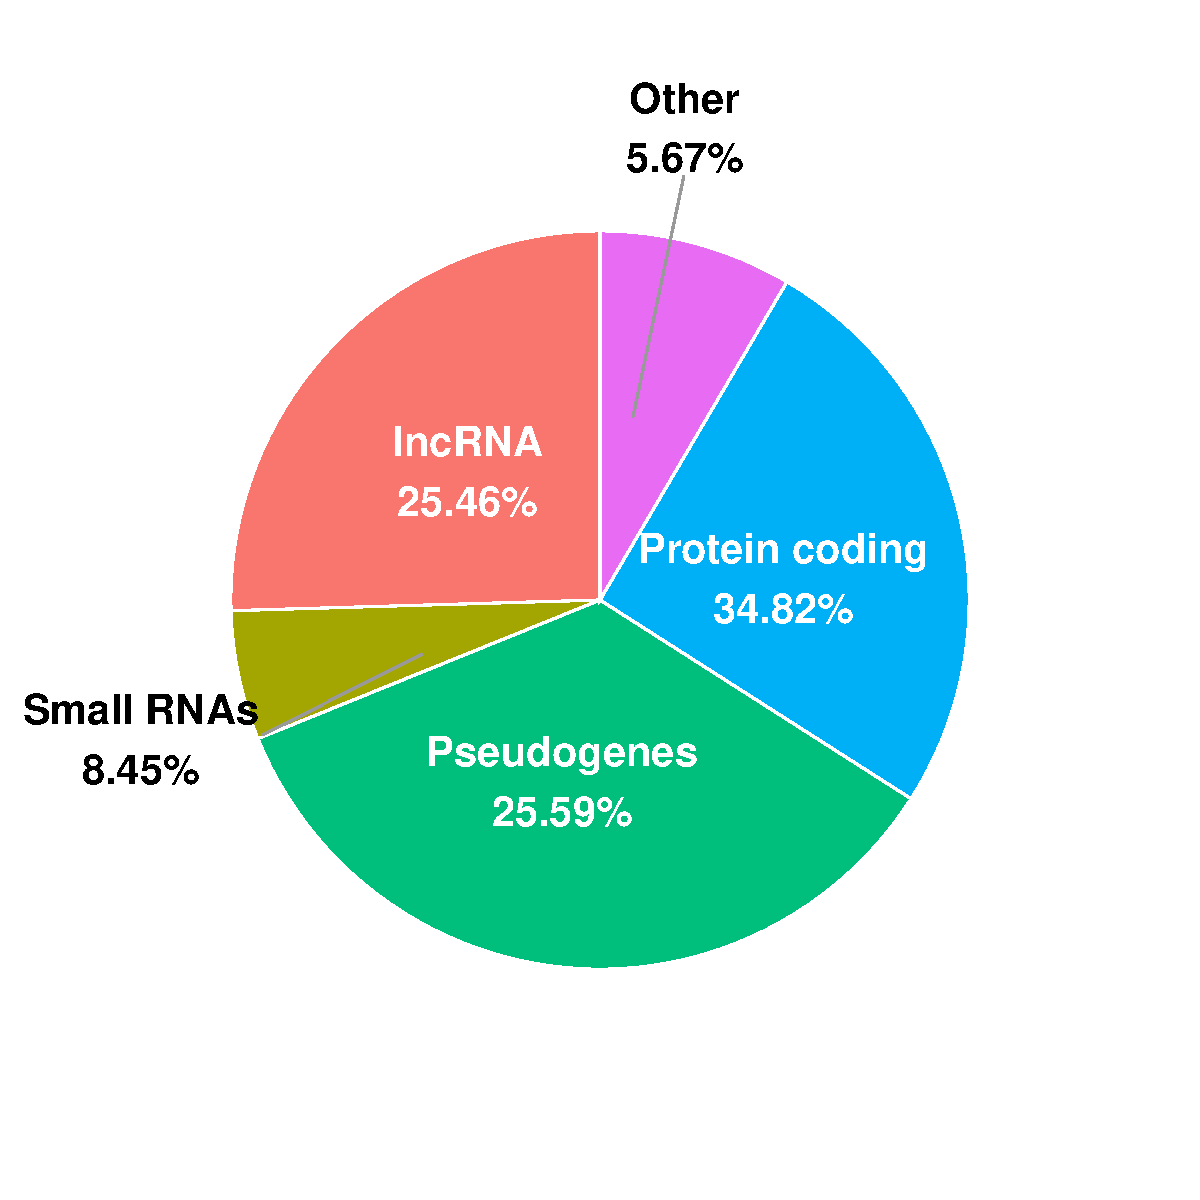
\includegraphics[keepaspectratio]{Final-Project-Quarto-Document_files/figure-pdf/fig-rna-type-1.pdf}}

}

\caption{\label{fig-rna-type}Detected RNA Types. The number of genes
detected in each RNA category from RNA-seq data were counted and plotted
as a pie chart. Small categories (\textless{} 2 \%), such as rRNA, tRNA,
and immunoglobulin genes, were combined into an `Other' category.}

\end{figure}%

Figure 2. Expression by RNA Type (similar to figure 1 but expression
based rather than count based)

\begin{figure}

\centering{

\pandocbounded{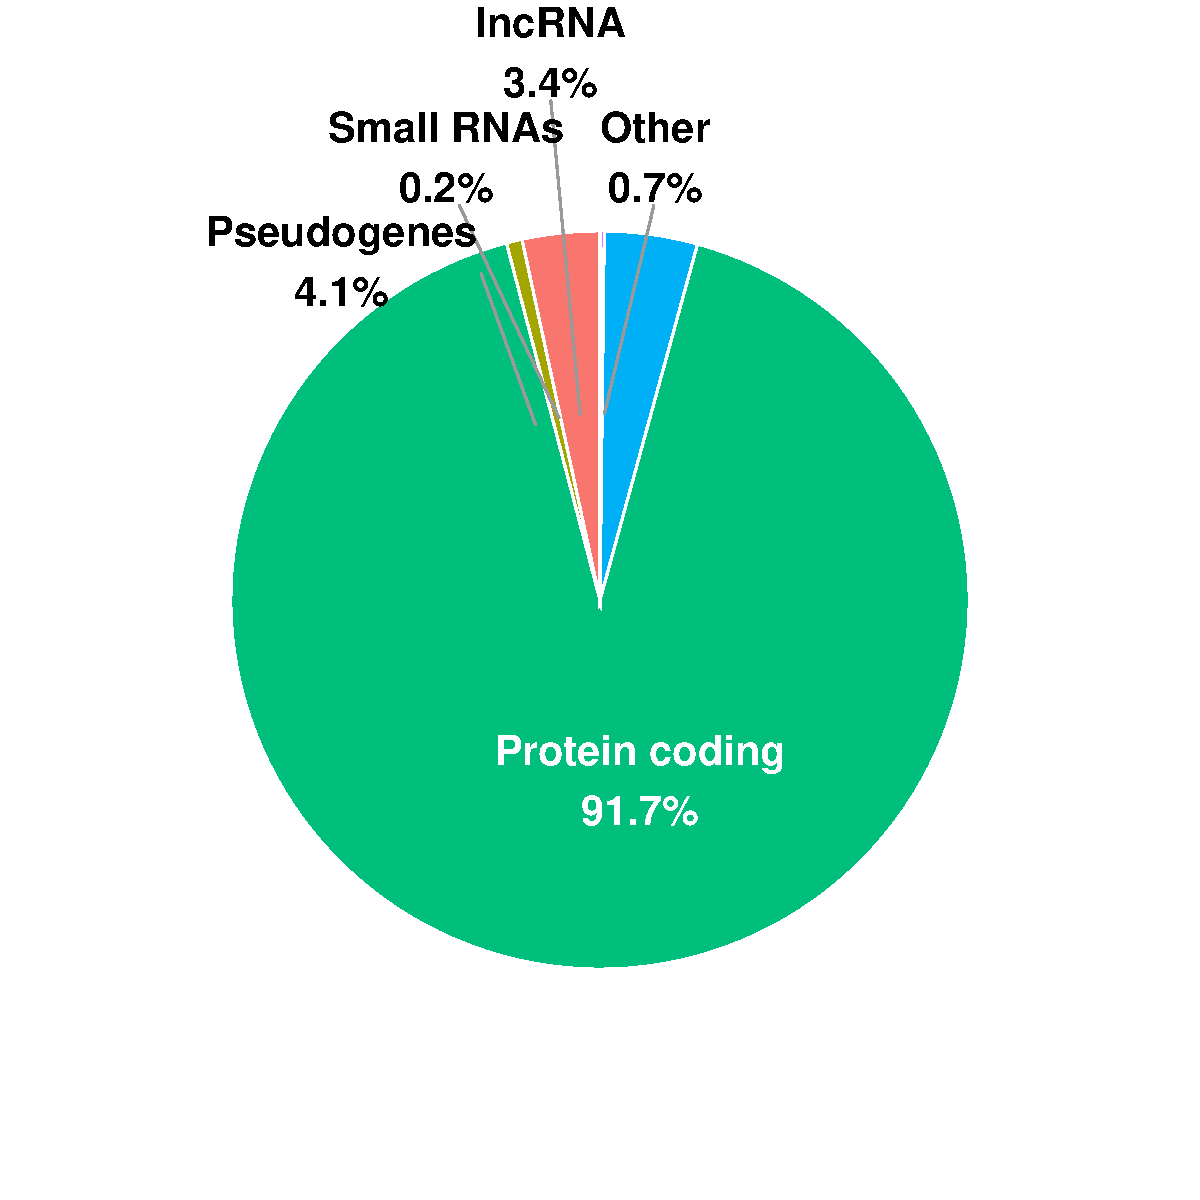
\includegraphics[keepaspectratio]{Final-Project-Quarto-Document_files/figure-pdf/fig-rna-expression-1.pdf}}

}

\caption{\label{fig-rna-expression}Expression by RNA Types. The
expression of genes, using raw count per million data, was averaged by
type of RNA and plotted as a pie chart. Small categories (\textless{} 2
\%), such as rRNA, tRNA, and immunoglobulin genes, were combined into an
`Other' category.}

\end{figure}%

\begin{verbatim}
[1] TRUE
\end{verbatim}

Figure 3. Expression of Pluripotency Genes (SOX2, POU5F1(OCT4), KLF4,
MYC (c-Myc), TRA-1-81 and 1-60 (PODXL), NANOG, FUT4 (SSEA4), LIN28A,
LIN28B, ESRRB, PRDM14, ZRP42 (REX1), TFCP2L1

(ectoderm: PAX6, NESTIN or SOX1 (neural projenitor/stem cell markers),
KRT14 (epithelial), endoderm: SOX17, AFP (hepatic), PDX1 (pancreatic),
mesoderm: CD34 (hematopoitic), CD90 (mesenchymal), NKX2.5 (cardiac
progenitor))

\begin{Shaded}
\begin{Highlighting}[]
\CommentTok{\#create a list of pluripotency, differentiation, and housekeeping genes}
\NormalTok{pluripotency\_genes }\OtherTok{\textless{}{-}} \FunctionTok{c}\NormalTok{(}\StringTok{"SOX2"}\NormalTok{, }\StringTok{"POU5F1"}\NormalTok{, }\StringTok{"KLF4"}\NormalTok{, }\StringTok{"MYC"}\NormalTok{,}
                        \StringTok{"PODXL"}\NormalTok{, }\StringTok{"NANOG"}\NormalTok{, }\StringTok{"FUT4"}\NormalTok{, }\StringTok{"LIN28A"}\NormalTok{, }
                        \StringTok{"LIN28B"}\NormalTok{, }\StringTok{"ESRRB"}\NormalTok{, }\StringTok{"PRDM14"}\NormalTok{, }\StringTok{"TFCP2L1"}\NormalTok{)}

\NormalTok{differentiation\_genes }\OtherTok{\textless{}{-}} \FunctionTok{c}\NormalTok{(}\StringTok{"SOX1"}\NormalTok{,}\StringTok{"PAX6"}\NormalTok{,}\StringTok{"NESTIN"}\NormalTok{,}\StringTok{"KRT14"}\NormalTok{, }
                           \StringTok{"SOX17"}\NormalTok{, }\StringTok{"AFP"}\NormalTok{, }\StringTok{"PDX1"}\NormalTok{, }\StringTok{"CD34"}\NormalTok{, }
                           \StringTok{"CD90"}\NormalTok{, }\StringTok{"NKX2.5"}\NormalTok{)}

\NormalTok{housekeeping\_genes }\OtherTok{\textless{}{-}} \FunctionTok{c}\NormalTok{(}\StringTok{"ACTB"}\NormalTok{,}\StringTok{"GAPDH"}\NormalTok{,}\StringTok{"RPL13A"}\NormalTok{,}\StringTok{"HPRT1"}\NormalTok{,}
                        \StringTok{"B2M"}\NormalTok{,}\StringTok{"TBP"}\NormalTok{,}\StringTok{"PGK1"}\NormalTok{,}\StringTok{"UBC"}\NormalTok{, }\StringTok{"RPL36AL"}\NormalTok{)}
\end{Highlighting}
\end{Shaded}

\begin{figure}

\centering{

\pandocbounded{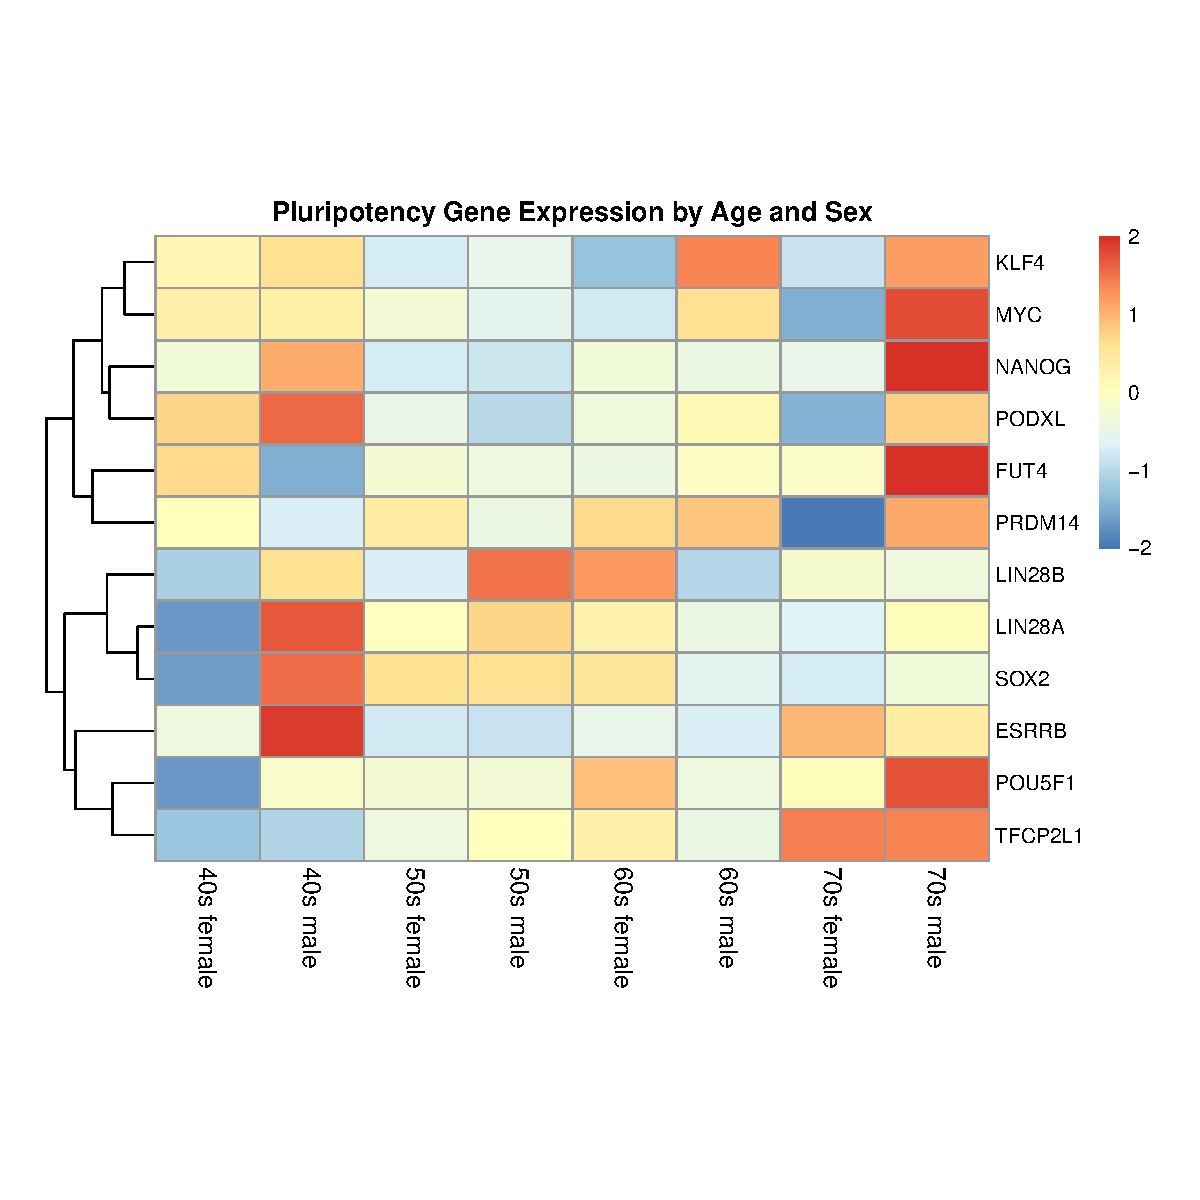
\includegraphics[keepaspectratio]{Final-Project-Quarto-Document_files/figure-pdf/fig-pluripotency-1.pdf}}

}

\caption{\label{fig-pluripotency}Expression of Pluripotency Genes}

\end{figure}%

\begin{figure}

\centering{

\pandocbounded{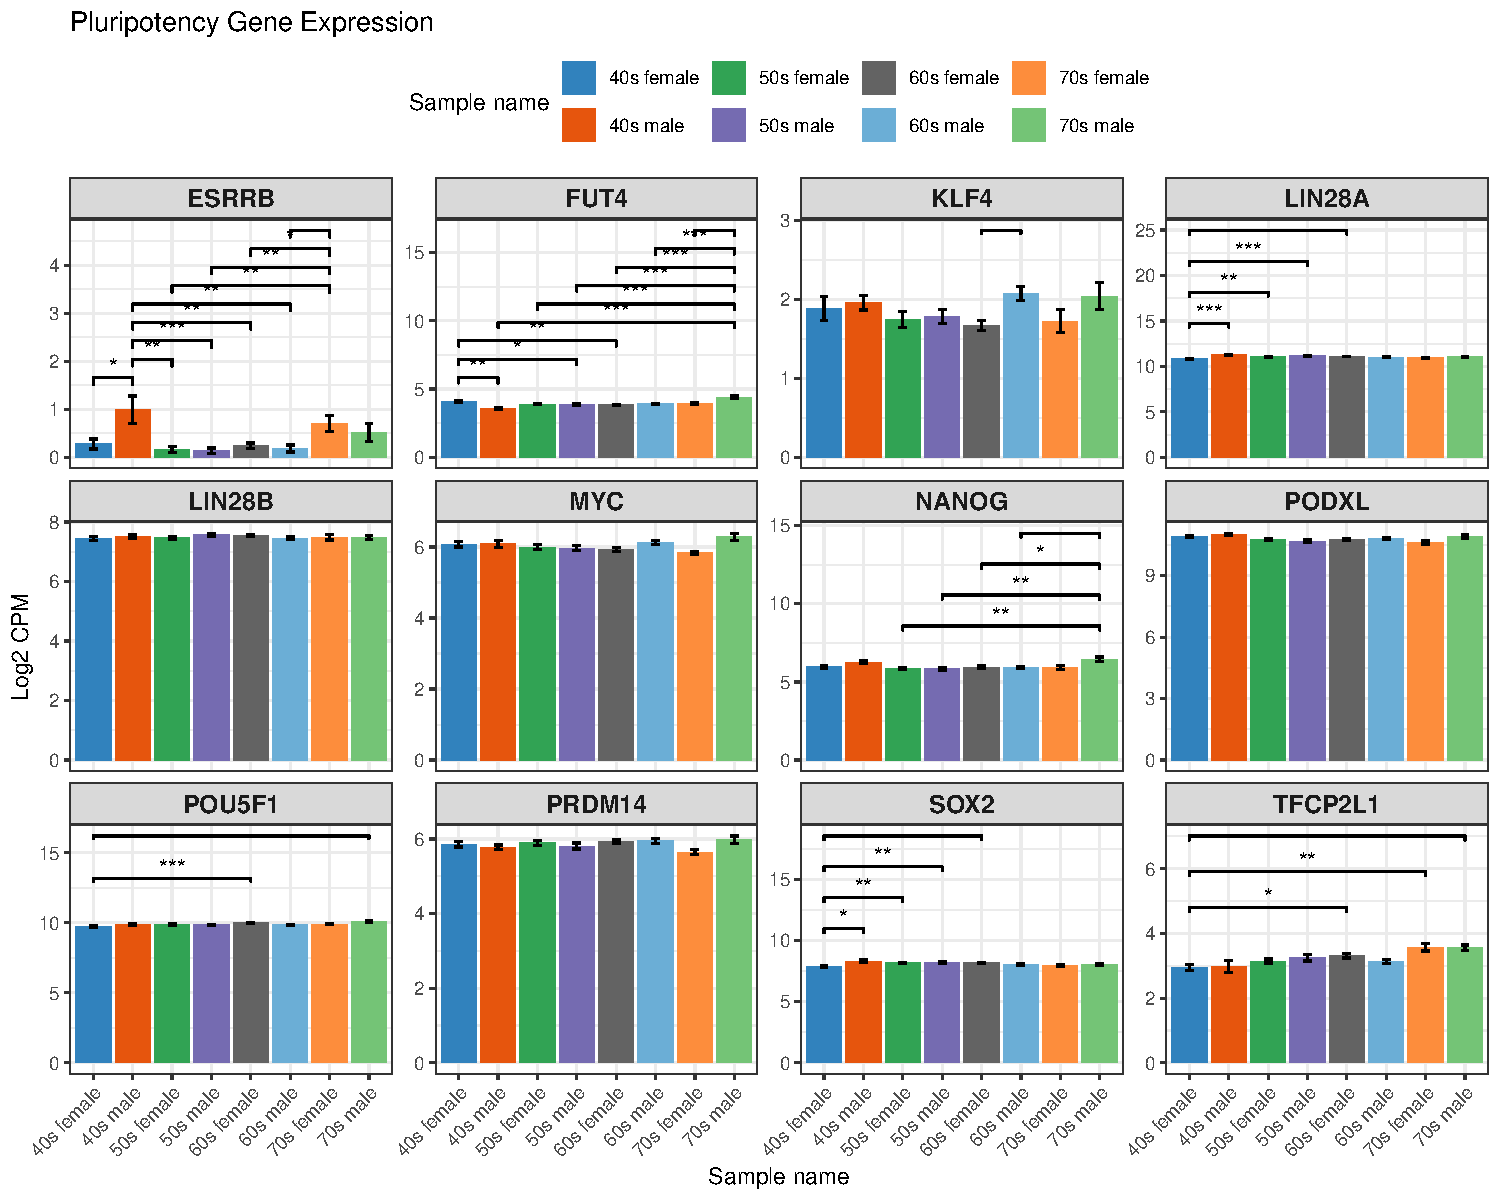
\includegraphics[keepaspectratio]{Final-Project-Quarto-Document_files/figure-pdf/fig-pluripotency2-1.pdf}}

}

\caption{\label{fig-pluripotency2}Expression of Pluripotency Genes}

\end{figure}%

\begin{verbatim}
character(0)
\end{verbatim}

\begin{verbatim}
Linear mixed model fit by REML. t-tests use Satterthwaite's method [
lmerModLmerTest]
Formula: Expression ~ sex + age_decade + (1 | `Gene name`)
   Data: logCPM_pluripotency

REML criterion at convergence: 4860

Scaled residuals: 
    Min      1Q  Median      3Q     Max 
-4.5766 -0.5524  0.0324  0.5434  5.6678 

Random effects:
 Groups    Name        Variance Std.Dev.
 Gene name (Intercept) 12.0276  3.4681  
 Residual               0.2103  0.4586  
Number of obs: 3696, groups:  Gene name, 12

Fixed effects:
                Estimate Std. Error         df t value Pr(>|t|)    
(Intercept)      6.18060    1.00136   11.00810   6.172 6.96e-05 ***
sexmale          0.03648    0.01574 3680.00000   2.318   0.0205 *  
age_decade50s   -0.02250    0.02441 3680.00000  -0.922   0.3568    
age_decade60s    0.01016    0.02370 3680.00000   0.429   0.6681    
age_decade70s    0.08018    0.03245 3680.00000   2.471   0.0135 *  
---
Signif. codes:  0 '***' 0.001 '**' 0.01 '*' 0.05 '.' 0.1 ' ' 1

Correlation of Fixed Effects:
            (Intr) sexmal ag_d50 ag_d60
sexmale     -0.003                     
age_decd50s -0.017 -0.131              
age_decd60s -0.017 -0.156  0.742       
age_decd70s -0.013 -0.098  0.540  0.558
\end{verbatim}

\begin{verbatim}
Type III Analysis of Variance Table with Satterthwaite's method
           Sum Sq Mean Sq NumDF DenDF F value   Pr(>F)   
sex        1.1296 1.12964     1  3680  5.3721 0.020516 * 
age_decade 2.8948 0.96492     3  3680  4.5887 0.003278 **
---
Signif. codes:  0 '***' 0.001 '**' 0.01 '*' 0.05 '.' 0.1 ' ' 1
\end{verbatim}

\begin{verbatim}
$emmeans
 age_decade emmean SE  df asymp.LCL asymp.UCL
 40s          6.20  1 Inf      4.24      8.16
 50s          6.18  1 Inf      4.21      8.14
 60s          6.21  1 Inf      4.25      8.17
 70s          6.28  1 Inf      4.32      8.24

Results are averaged over the levels of: sex 
Degrees-of-freedom method: asymptotic 
Confidence level used: 0.95 

$contrasts
 contrast  estimate     SE  df z.ratio p.value
 40s - 50s   0.0225 0.0244 Inf   0.922  0.7933
 40s - 60s  -0.0102 0.0237 Inf  -0.429  0.9736
 40s - 70s  -0.0802 0.0325 Inf  -2.471  0.0646
 50s - 60s  -0.0327 0.0173 Inf  -1.887  0.2335
 50s - 70s  -0.1027 0.0282 Inf  -3.643  0.0015
 60s - 70s  -0.0700 0.0275 Inf  -2.545  0.0533

Results are averaged over the levels of: sex 
Degrees-of-freedom method: asymptotic 
P value adjustment: tukey method for comparing a family of 4 estimates 
\end{verbatim}

\begin{verbatim}
$emmeans
 sex    emmean SE  df asymp.LCL asymp.UCL
 female   6.20  1 Inf      4.24      8.16
 male     6.23  1 Inf      4.27      8.20

Results are averaged over the levels of: age_decade 
Degrees-of-freedom method: asymptotic 
Confidence level used: 0.95 

$contrasts
 contrast      estimate     SE  df z.ratio p.value
 female - male  -0.0365 0.0157 Inf  -2.318  0.0205

Results are averaged over the levels of: age_decade 
Degrees-of-freedom method: asymptotic 
\end{verbatim}

Fixed effects Sex effect (male): Expression is slightly higher in males
by 0.036 logCPM; significant at p = 0.0196.

Age effects: Only the 70s group is significantly higher than 40s (p =
0.0125). 50s and 60s are not significantly different from 40s.

Type III Analysis of Variance Table with Satterthwaite's method -
confirms both sex and age\_decade have a significant effect on
pluripotency gene expression when averaged across all genes.

Predicted mean logCPM expression (adjusted means, not raw means)

age\_decade emmean 40s 6.20 50s 6.18 60s 6.21 70s 6.28

Overall, pluripotency gene expression is slightly higher in males
compared to females, regardless of age. Expression also shows an
increasing trend with age, with samples from individuals in their 70s
being significantly higher than those from individuals in their 40s.
Differences between other age decades (50s, 60s) and 40s were not
statistically significant.

\begin{Shaded}
\begin{Highlighting}[]
\CommentTok{\#ANOVA and Tukey HSD}

\CommentTok{\#create empty dataframes to store results}
\NormalTok{gene\_anova\_results }\OtherTok{\textless{}{-}} \FunctionTok{data.frame}\NormalTok{()}
\NormalTok{gene\_tukey\_results }\OtherTok{\textless{}{-}} \FunctionTok{data.frame}\NormalTok{()}

\CommentTok{\#use a for loop to loop through each gene and perform an ANOVa and tukey tests}
\ControlFlowTok{for}\NormalTok{ (g }\ControlFlowTok{in} \FunctionTok{unique}\NormalTok{(logCPM\_pluripotency}\SpecialCharTok{$}\StringTok{\textasciigrave{}}\AttributeTok{Gene name}\StringTok{\textasciigrave{}}\NormalTok{)) \{}
  
\NormalTok{  gene\_data }\OtherTok{\textless{}{-}}\NormalTok{ logCPM\_pluripotency }\SpecialCharTok{\%\textgreater{}\%}
    \FunctionTok{filter}\NormalTok{(}\StringTok{\textasciigrave{}}\AttributeTok{Gene name}\StringTok{\textasciigrave{}} \SpecialCharTok{==}\NormalTok{ g)}
  
  \CommentTok{\# One{-}way ANOVA (Expression \textasciitilde{} sex\_age)}
\NormalTok{  fit }\OtherTok{\textless{}{-}} \FunctionTok{aov}\NormalTok{(Expression }\SpecialCharTok{\textasciitilde{}}\NormalTok{ age\_sex, }\AttributeTok{data =}\NormalTok{ gene\_data)}
  
  \CommentTok{\# Save tidy ANOVA table}
\NormalTok{  anova\_tbl }\OtherTok{\textless{}{-}}\NormalTok{ broom}\SpecialCharTok{::}\FunctionTok{tidy}\NormalTok{(fit) }\SpecialCharTok{\%\textgreater{}\%}
    \FunctionTok{mutate}\NormalTok{(}\AttributeTok{Gene =}\NormalTok{ g)}
  
\NormalTok{  gene\_anova\_results }\OtherTok{\textless{}{-}} \FunctionTok{rbind}\NormalTok{(gene\_anova\_results, anova\_tbl)}
  
  \CommentTok{\# Tukey HSD post{-}hoc for age\_sex}
\NormalTok{  tukey }\OtherTok{\textless{}{-}} \FunctionTok{TukeyHSD}\NormalTok{(fit, }\StringTok{"age\_sex"}\NormalTok{)}
\NormalTok{  tukey\_df }\OtherTok{\textless{}{-}} \FunctionTok{as.data.frame}\NormalTok{(tukey}\SpecialCharTok{$}\NormalTok{age\_sex) }\SpecialCharTok{\%\textgreater{}\%}
    \FunctionTok{rename}\NormalTok{(}\AttributeTok{p\_value =} \StringTok{\textasciigrave{}}\AttributeTok{p adj}\StringTok{\textasciigrave{}}\NormalTok{) }\SpecialCharTok{\%\textgreater{}\%} 
    \FunctionTok{mutate}\NormalTok{(}\AttributeTok{Gene =}\NormalTok{ g,}
           \AttributeTok{comparison =} \FunctionTok{rownames}\NormalTok{(.))}
  
\NormalTok{  gene\_tukey\_results }\OtherTok{\textless{}{-}} \FunctionTok{rbind}\NormalTok{(gene\_tukey\_results, tukey\_df)}
\NormalTok{\}}

\CommentTok{\# ANOVA FDR correction}
\NormalTok{pluripotency\_gene\_anova\_results }\OtherTok{\textless{}{-}}\NormalTok{ gene\_anova\_results }\SpecialCharTok{\%\textgreater{}\%}
  \FunctionTok{group\_by}\NormalTok{(term) }\SpecialCharTok{\%\textgreater{}\%}
  \FunctionTok{mutate}\NormalTok{(}\AttributeTok{p\_adj =} \FunctionTok{p.adjust}\NormalTok{(p.value, }\AttributeTok{method =} \StringTok{"BH"}\NormalTok{)) }\SpecialCharTok{\%\textgreater{}\%}
  \FunctionTok{ungroup}\NormalTok{()}

\CommentTok{\# Tukey HSD p{-}value adjustment}
\NormalTok{pluripotency\_gene\_tukey\_results }\OtherTok{\textless{}{-}}\NormalTok{ gene\_tukey\_results }\SpecialCharTok{\%\textgreater{}\%}
  \FunctionTok{group\_by}\NormalTok{(Gene) }\SpecialCharTok{\%\textgreater{}\%}
  \FunctionTok{mutate}\NormalTok{(}\AttributeTok{p\_adj =} \FunctionTok{p.adjust}\NormalTok{(p\_value, }\AttributeTok{method =} \StringTok{"BH"}\NormalTok{))  }

\CommentTok{\#see the number of p values less than 0.05}
\CommentTok{\#sum(gene\_tukey\_results$p\_value \textless{} 0.05, na.rm = TRUE)}
\end{Highlighting}
\end{Shaded}

\begin{figure}

\centering{

\pandocbounded{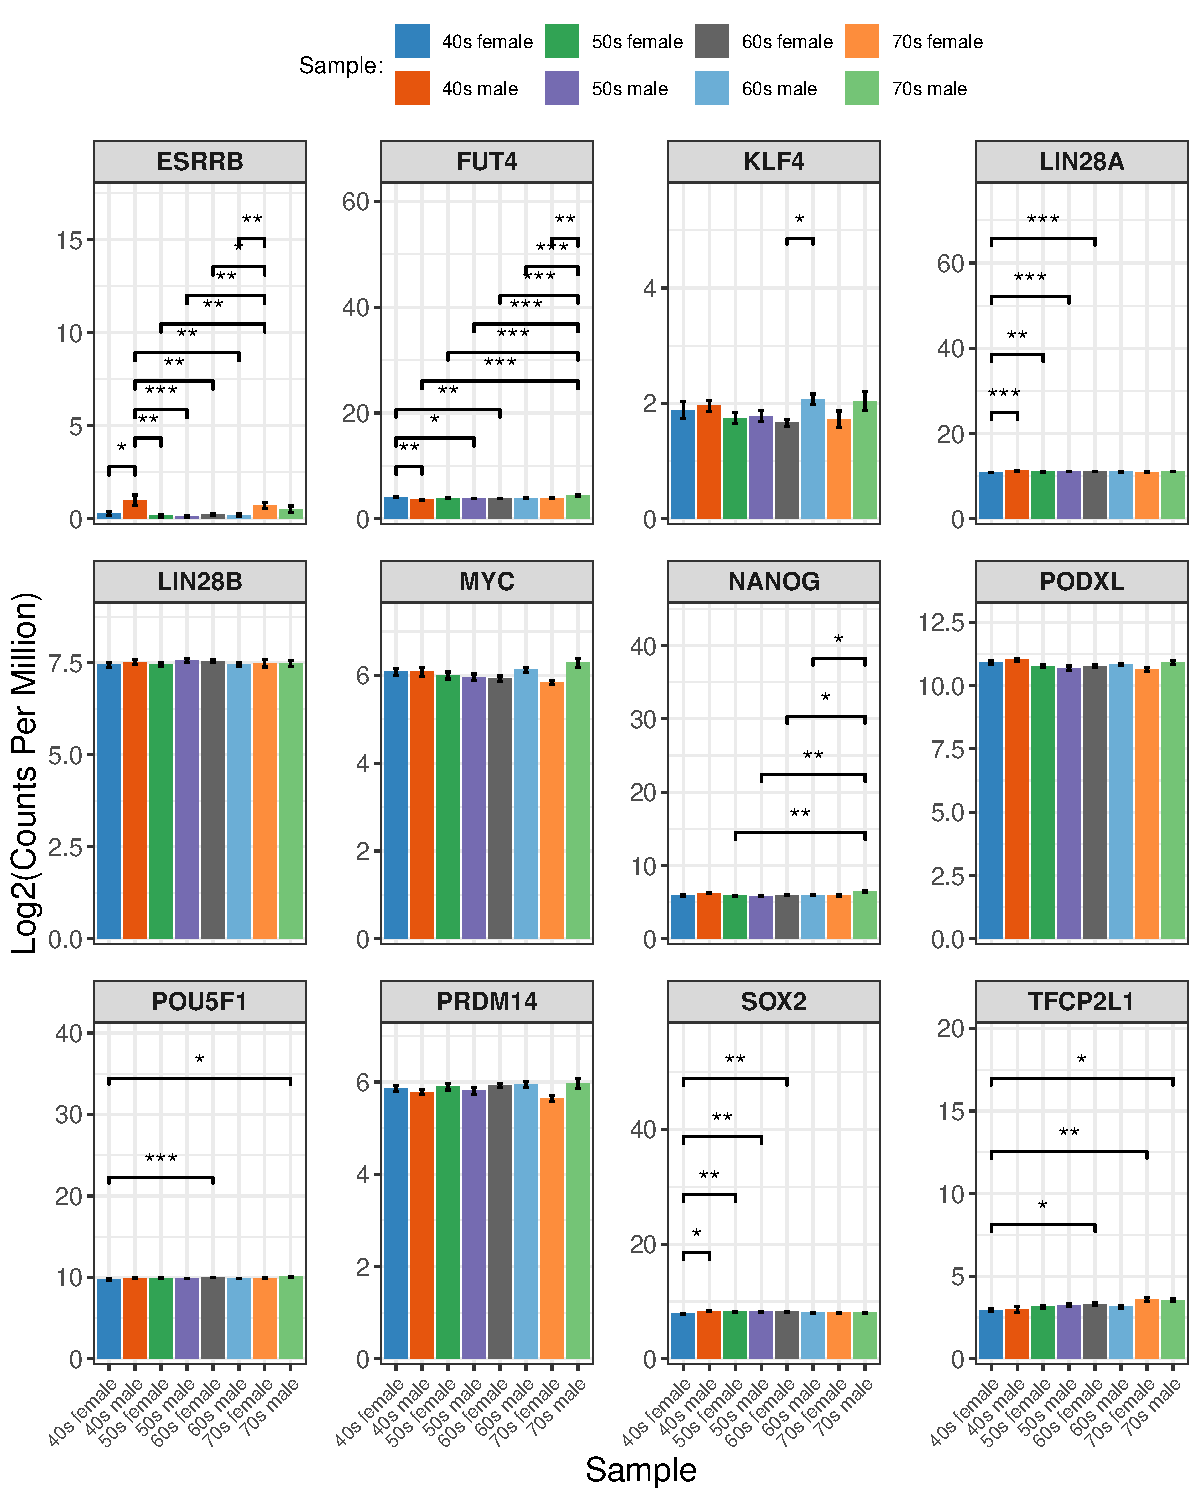
\includegraphics[keepaspectratio]{Final-Project-Quarto-Document_files/figure-pdf/fig-bargraph-pluripotency-1.pdf}}

}

\caption{\label{fig-bargraph-pluripotency}Pluripotency Gene Expression
by Age and Sex.}

\end{figure}%

Figure 4. Expression of Differentiation Genes (ectoderm: PAX6, NESTIN or
SOX1 (neural projenitor/stem cell markers), KRT14 (epithelial),
endoderm: SOX17, AFP (hepatic), PDX1 (pancreatic), mesoderm: CD34
(hematopoitic), CD90 (mesenchymal), NKX2.5 (cardiac progenitor))

Figure 5. Expression of Housekeeping Genes (some sort of general figure
or sorted by housekeeping type (i.e.~ribosomal, metabolic, cytoskeleton,
etc.))

Figure 6. Expression of Housekeeping Genes (focusing on some genes,
either over time during reprogramming or across different conditions)

these figures may be split into more than the six described depending on
the data

figures will include heat maps, bar charts, and possibly volcano plots

\section{Discussion}\label{discussion}

\section{Conclusion}\label{conclusion}

\begin{center}\rule{0.5\linewidth}{0.5pt}\end{center}

\section*{References}\label{references}
\addcontentsline{toc}{section}{References}

\phantomsection\label{refs}
\begin{CSLReferences}{1}{0}
\bibitem[\citeproctext]{ref-artyukhov2017}
Artyukhov, A. S., Dashinimaev, E. B., Tsvetkov, V. O., Bolshakov, A. P.,
Konovalova, E. V., Kolbaev, S. N., Vorotelyak, E. A. \& Vasiliev, A. V.
(2017). New genes for accurate normalization of qRT-PCR results in study
of iPS and iPS-derived cells. \emph{Gene}, \emph{626}, 234--240.
\url{https://doi.org/10.1016/j.gene.2017.05.045}

\bibitem[\citeproctext]{ref-carcamo-orive2017}
Carcamo-Orive, I., Hoffman, G. E., Cundiff, P., Beckmann, N. D.,
D'Souza, S. L., Knowles, J. W., Patel, A., Papatsenko, D., Abbasi, F.,
Reaven, G. M., Whalen, S., Lee, P., Shahbazi, M., Henrion, M. Y. R.,
Zhu, K., Wang, S., Roussos, P., Schadt, E. E., Pandey, G., \ldots{}
Lemischka, I. (2017). Analysis of Transcriptional Variability in a Large
Human iPSC Library Reveals Genetic and Non-genetic Determinants of
Heterogeneity. \emph{Cell Stem Cell}, \emph{20}(4), 518--532.e9.
\url{https://doi.org/10.1016/j.stem.2016.11.005}

\bibitem[\citeproctext]{ref-cerneckis2024}
Cerneckis, J., Cai, H. \& Shi, Y. (2024). Induced pluripotent stem cells
(iPSCs): molecular mechanisms of induction and applications.
\emph{Signal Transduction and Targeted Therapy}, \emph{9}(1), 112.
\url{https://doi.org/10.1038/s41392-024-01809-0}

\bibitem[\citeproctext]{ref-ensembl}
\emph{Ensembl biomart}. (n.d.).
\url{https://www.ensembl.org/biomart/martview/95a58994f7c82fc6f316078faa7f92e7}

\bibitem[\citeproctext]{ref-panina2020}
Panina, Y., Germond, A. \& Watanabe, T. M. (2020). Analysis of the
stability of 70 housekeeping genes during iPS reprogramming.
\emph{Scientific Reports}, \emph{10}, 21711.
\url{https://doi.org/10.1038/s41598-020-78863-5}

\bibitem[\citeproctext]{ref-poetsch2022}
Poetsch, M. S., Strano, A. \& Guan, K. (2022). Human induced pluripotent
stem cells: From cell origin, genomic stability, and epigenetic memory
to translational medicine. \emph{Stem Cells}, \emph{40}(6), 546--555.
\url{https://doi.org/10.1093/stmcls/sxac020}

\bibitem[\citeproctext]{ref-stemform}
\emph{Stemformatics datasets}. (n.d.).
\url{https://www.stemformatics.org/datasets/view?id=7274}

\bibitem[\citeproctext]{ref-takahashi2007}
Takahashi, K., Tanabe, K., Ohnuki, M., Narita, M., Ichisaka, T., Tomoda,
K. \& Yamanaka, S. (2007). Induction of pluripotent stem cells from
adult human fibroblasts by defined factors. \emph{Cell}, \emph{131}(5),
861--872. \url{https://doi.org/10.1016/j.cell.2007.11.019}

\bibitem[\citeproctext]{ref-wang2009}
Wang, Z., Gerstein, M. \& Snyder, M. (2009). RNA-seq: A revolutionary
tool for transcriptomics. \emph{Nature Reviews. Genetics}, \emph{10}(1),
57--63. \url{https://doi.org/10.1038/nrg2484}

\bibitem[\citeproctext]{ref-R-tidyverse}
Wickham, H. (2023). \emph{Tidyverse: Easily install and load the
tidyverse}. \url{https://tidyverse.tidyverse.org}

\bibitem[\citeproctext]{ref-R-ggplot2}
Wickham, H., Chang, W., Henry, L., Pedersen, T. L., Takahashi, K.,
Wilke, C., Woo, K., Yutani, H., Dunnington, D. \& van den Brand, T.
(2025). \emph{ggplot2: Create elegant data visualisations using the
grammar of graphics}. \url{https://ggplot2.tidyverse.org}

\bibitem[\citeproctext]{ref-R-dplyr}
Wickham, H., François, R., Henry, L., Müller, K. \& Vaughan, D. (2023).
\emph{Dplyr: A grammar of data manipulation}.
\url{https://dplyr.tidyverse.org}

\bibitem[\citeproctext]{ref-R-scales}
Wickham, H., Pedersen, T. L. \& Seidel, D. (2025). \emph{Scales: Scale
functions for visualization}. \url{https://scales.r-lib.org}

\end{CSLReferences}




\end{document}
